\documentclass{ctexbook}
\usepackage[utf8]{inputenc}
\usepackage{hyperref, bookmark}
\usepackage{amsmath}
\usepackage{amssymb}
\usepackage{amsfonts}
\usepackage{amsthm}

\ctexset{
    chapter = {
        number = \arabic{chapter},
    },
    section = {
        name = {\S,},
        number = \arabic{section},
    },
    subsection = {
        name = {},
        number = {},
        aftername = {},
    },
}

\newcommand{\problem}[1]{\subsection{第 {#1} 题}}
% 使公式编号与小节关联
\numberwithin{equation}{section}
% \makeatletter
% \@addtoreset{equation}{section}
% \makeatother

\newcommand{\abdet}[1]{\begin{vmatrix}#1\end{vmatrix}}

\newtheorem{lemma}{引理}[section]

\newcommand{\abref}[1]{式 \eqref{#1}}
\newcommand{\lemmaref}[1]{引理 \ref{#1}}

\newcommand{\setN}{\mathbb{N}}
\newcommand{\setZ}{\mathbb{Z}}

\title{《代数学引论(第一卷)》(柯斯特利金)习题}
\author{Abreto Fu\footnote{Email:~abreto [AT] std.uestc.edu.cn}}

\begin{document}

\pdfbookmark[chapter]{标题页}{title}
\maketitle

\cleardoublepage
\pdfbookmark[chapter]{\contentsname}{toc}
\tableofcontents

% Chapter 01
\cleardoublepage

\chapter{代数的起源}

\section{简谈代数}

\section{几个典型问题}

\section{线性方程初步}

\section{低阶行列式}

\problem{2}
\begin{quotation}
    证明在三阶行列式展开式中的六项不可能同时为正.
\end{quotation}

\begin{proof}

展开式中的六项的乘积为
\begin{equation}\label{eq:ch01:sec04:prob02}
\begin{aligned}
    \Gamma &= a_{11}a_{22}a_{33}\cdot{}a_{12}a_{23}a_{31}\cdot{a_{13}}a_{21}a_{32} \\
    & \qquad \cdot(-a_{11}a_{23}a_{32})\cdot(-a_{12}a_{21}a_{33})\cdot(-a_{13}a_{22}a_{31}) \\
    &= -(a_{11}a_{12}a_{13}a_{21}a_{22}a_{23}a_{31}a_{32}a_{33})^2 \le 0
\end{aligned}
\end{equation}

若这六项同时为正,则应有
\begin{equation}
    \Gamma > 0
\end{equation}

与\abref{eq:ch01:sec04:prob02} 矛盾.

故在三阶行列式展开式中的六项不可能同时为正.

\end{proof}

\problem{3}
\begin{quotation}
验证
\[
\begin{vmatrix}
    a_{11} & a_{12} & a_{13} \\
    a_{21} & a_{22} & a_{23} \\
    a_{31} & a_{32} & a_{33}
\end{vmatrix}
=
\begin{vmatrix}
    a_{11} & a_{21} & a_{31} \\
    a_{12} & a_{22} & a_{32} \\
    a_{13} & a_{23} & a_{33}
\end{vmatrix}
, \quad
\begin{vmatrix}
    0 & a & b \\
    -a & 0 & c \\
    -b & -c & 0
\end{vmatrix}
= 0.
\]
\end{quotation}

\begin{lemma}\label{lem:ch01:sec04:lem1}
    \[
        \begin{vmatrix}
            a & b \\ c & d
        \end{vmatrix}
        =
        \begin{vmatrix}
            a & c \\ b & d
        \end{vmatrix}
    \]
\end{lemma}
\lemmaref{lem:ch01:sec04:lem1} 可由定义直接导出.

\begin{lemma}\label{lem:ch01:sec04:2}
\[
    -a\begin{vmatrix} c & d \\ e & f \end{vmatrix}
    +b\begin{vmatrix} c & d \\ g & h \end{vmatrix}
    =
    -c\abdet{a & b \\ h & f}
    +d\abdet{a & b \\ g & e}
\]
\end{lemma}
\begin{proof}
\[
\begin{aligned}
    -a\abdet{c & d \\ e & f} + b\abdet{c & d \\ g & h}
    &= -a(cf - de) + b(ch - dg) \\
    &= -c(af - bh) + d(ae - bg) \\
    &= -c\abdet{a & b \\ h & f}+d\abdet{a & b \\ g & e}
\end{aligned}
\]
\end{proof}

\paragraph{第一个式子}

\begin{equation}
\begin{aligned}
    D_1 &= \abdet{a_{11} & a_{12} & a_{13} \\ a_{21} & a_{22} & a_{23} \\ a_{31} & a_{32} & a_{33}} \\
    &= a_{11}\abdet{a_{22} & a_{23} \\ a_{32} & a_{33}}
      -a_{21}\abdet{a_{12} & a_{13} \\ a_{32} & a_{33}}
      +a_{31}\abdet{a_{12} & a_{13} \\ a_{22} & a_{23}}
\end{aligned} 
\end{equation}

由\lemmaref{lem:ch01:sec04:lem1} 可知
\begin{equation}
    a_{11}\abdet{a_{22} & a_{23} \\ a_{32} & a_{33}}
    =
    a_{11}\abdet{a_{22} & a_{32} \\ a_{23} & a_{33}}
\end{equation}

由\lemmaref{lem:ch01:sec04:2} 得
\begin{equation}
    -a_{21}\abdet{a_{12} & a_{13} \\ a_{32} & a_{33}}
    +a_{31}\abdet{a_{12} & a_{13} \\ a_{22} & a_{23}}
    =
    -a_{12}\abdet{a_{21} & a_{31} \\ a_{23} & a_{33}}
    +a_{13}\abdet{a_{21} & a_{31} \\ a_{22} & a_{32}}
\end{equation}

于是
\begin{equation}
\begin{aligned}
    D_1 &= a_{11}\abdet{a_{22} & a_{32} \\ a_{23} & a_{33}}
    -a_{12}\abdet{a_{21} & a_{31} \\ a_{23} & a_{33}}
    +a_{13}\abdet{a_{21} & a_{31} \\ a_{22} & a_{32}} \\
    &= \abdet{
        a_{11} & a_{21} & a_{31} \\
        a_{12} & a_{22} & a_{32} \\
        a_{13} & a_{23} & a_{33}
    }
\end{aligned}
\end{equation}
第一个式子验证完毕.

\paragraph{第二个式子} % (fold)

\begin{equation}
\begin{aligned}
\abdet{
    0 & a & b \\
    -a & 0 & c \\
    -b & -c & 0
} &= 0\abdet{0 & c \\ -c & 0}
    -(-a)\abdet{a & b \\ -c & 0}
    +(-b)\abdet{a & b \\ 0 & c} \\
  &= abc - bac = 0
\end{aligned}
\end{equation}

验证完毕.

% paragraph 第二个式子 (end)

\section{集合与映射} % (begin)

\begin{lemma}\label{lem:ch01:sec05:1}
    设
    \[
        f: X \to Y, \qquad g: Y \to X
    \]
    是任意两个映射,如果 $gf = e_X$,则 $f$ 是单的,$g$ 是满的.
\end{lemma}

\problem{1}
\begin{quotation}
    设 $\Omega = \{+,-,++,+-,-+,--,+++,\cdots\}$ 是加号和减号的有限序列的集合,
    而 $f: \Omega \to \Omega$ 是一个变换,将元素
    $\omega = \omega_1\omega_2\cdots\omega_n\in\Omega$
    对应到
    $\omega' = \omega_1\dot{\omega}_1\omega_2\dot{\omega}_2\cdots\omega_n\dot{\omega}_n$,
    其中若 $\omega_k=+$,则 $\dot{\omega}_k=-$,
    若 $\omega_k=-$,则 $\dot{\omega}_k=+$.
    证明在 $f(f\omega)$ 的长度 $>4$ 的任意区间内包含 $++$ 或 $--$.
\end{quotation}

\begin{proof}
    设
    \begin{equation}
        f(f\omega) = \omega_0\omega_1\omega_2\cdots\omega_n
    \end{equation}

    由定义易知,
    \begin{equation}
        \forall k \ge 0, \omega_{4k+1} = \omega_{4k+2}
    \end{equation}

    对于任意长度 $>4$ 的区间,一定包含连续的两项形如 $\omega_{4k+1}\omega_{4k+2}$.

    即一定包含相等的连续两项.
\end{proof}

\problem{2}
\begin{quotation}
    由法则 $n \to n^2$ 给出的映射 $f: \setN \to \setN$ 有右逆吗?
    给出 $f$ 的两个左逆.
\end{quotation}

假设 $f$ 有右逆 $g$,即
\begin{equation}
    fg = e_\setN
\end{equation}
由\lemmaref{lem:ch01:sec05:1} 得,$f$ 是满的,
与题设矛盾.
故 $f$ 不存在右逆.

给出两个左逆如下
\begin{equation}
    h_1(n) = \begin{cases}
        \sqrt{n}, & n \text{ 是完全平方数}; \\
        1, & \text{otherwise}.
    \end{cases}
\end{equation}
\begin{equation}
    h_2(n) = \begin{cases}
        \sqrt{n}, & n \text{ 是完全平方数}; \\
        2, & \text{otherwise}.
    \end{cases}
\end{equation}

\problem{3}
\begin{quotation}
    设 $f: X \to Y$ 是一个映射,且 $S, T$ 都是 $X$ 的子集.

    证明
    \[
        f(S \cup T) = f(S) \cup f(T),
        \quad f(S \cap T) \subset f(S) \cap f(T).
    \]
    试举一例,说明后一个式子中的包含关系一般来说不能换成相等关系.
\end{quotation}

\paragraph{第一个式子} % (fold)
\label{par:第一个式子}
\begin{proof}
    \begin{equation}
        \forall y \in f(S \cup T),
        \exists x \in S \cup T,
        f(x) = y.
    \end{equation}
    \begin{enumerate}
        \item $x \in S$,则 $y = f(x) \in S;$
        \item $x \in T$,则 $y = f(x) \in T.$
    \end{enumerate}
    于是
    \begin{equation}
        f(S \cup T) \subset f(S) \cup f(T).
    \end{equation}

    \begin{equation}
        \forall y \in f(S) \cup f(T),
        \text{ 要么}\: y \in f(S),
        \text{ 要么}\: y \in f(T).
    \end{equation}
    \begin{enumerate}
        \item $y \in f(S)$,则 $\exists x \in S \subset S \cup T, f(x) = y$,
            于是 $y \in f(S \cup T);$
        \item $y \in f(T)$,则 $\exists x \in T \subset S \cup T, f(x) = y$,
            于是 $y \in f(S \cup T).$
    \end{enumerate}
    所以
    \begin{equation}
        f(S) \cup f(T) \subset f(S \cup T).
    \end{equation}

    综上所述
    \begin{equation}
        f(S \cup T) = f(S) \cup f(T)
    \end{equation}
\end{proof}
% paragraph 第一个式子 (end)

\paragraph{第二个式子} % (fold)
\label{par:第二个式子}
\begin{proof}
    \begin{equation}
        \forall y \in f(S \cap T),
        \exists x \in S \cap T,
        f(x) = y.
    \end{equation}

    此时 $x \in S$ 且 $x \in T$,
    所以 $f(x) \in f(S)$ 且 $f(x) \in f(T)$,
    即 $y = f(x) \in f(S) \cap f(T)$.

    故而
    \begin{equation}
        f(S \cap T) \subset f(S) \cap f(T).
    \end{equation}
\end{proof}
% paragraph 第二个式子 (end)

\paragraph{一个反例} % (fold)
\label{par:一个反例}
考虑映射 $f: n \mapsto n^2$,
以及 $\setZ$ 的子集 $S = \{-1, 0\}, T = \{0, 1\}$.

那么
\begin{equation}
    S \cap T = \{ 0 \}, \quad f(S \cap T) = \{ 0 \},
\end{equation}
同时
\begin{equation}
    f(S) = \{ 1, 0 \}, f(T) = \{ 0, 1 \},
    \quad f(S) \cap f(T) = \{ 0, 1 \}.
\end{equation}

在这种情况下,
$f(S) \cap f(T) \nsubseteq f(S \cap T)$.
所以包含关系不能换成相等关系.
% paragraph 一个反例 (end)

\problem{4} % (begin)
\begin{quotation}
    集合 $S$ 的全体子集的集合记做
    \begin{equation*}
        \mathcal{P}(S) = \{ T \vert T \subset S \}
    \end{equation*}
    假如若 $S=\{s_1,s_2,\cdots,s_n\}$ 是含有 $n$ 个元素的有限集,
    则 $\mathcal{P}(S)$ 由空集 $\varnothing,$
    $n$ 个单元集 $\{s_1\}, \{s_2\}, \cdots, \{s_n\},$
    $n(n-1)/2$ 个二元集 $\{s_i, s_j\}, 1 \le i < j \le n,$
    等等,直到全集 $T = S$ 组成.
    集合 $\mathcal{P}(S)$ 的基数是多少?
\end{quotation}

$\mathcal{P}(S)$ 的基数即为 $S$ 的不同子集的个数,
也是从 $S$ 中选取若干个元素出来的方案数.

每次选择对每个元素来说有选与不选两种可能,
于是总的方案数为 $2^n$,即
\begin{equation}
    \vert \mathcal{P}(S) \vert = 2^n.
\end{equation}
% problem 4 (end)

\problem{5} % (begin)
\begin{quotation}
    设 $f: X \to Y$ 是一个映射,
    且设对某个元素 $a \in X, b = f(a)$.
    原像
    \[
        f^{-1}(b) = f^{-1}(f(a)) = \{ x \vert f(x) = f(a) \}
    \]
    叫作元素 $b \in \mathrm{Im}f$ 上的纤维.
    证明集合 $X$ 是互不相交的纤维的并(也就是说,
    给出了 $X$ 的一个划分).
\end{quotation}
\begin{proof}
    设任意 $b_1, b_2 \in \mathrm{Im}f$ 且 $b_1 \ne b_2$,
    则 $f^{-1}(b_1) \cap f^{-1}(b_2) = \varnothing$,
    否则将有 $b_1 = b_2$,与前述矛盾.

    下面证明
    \begin{equation*}
        X = \bigcup_{b \in \mathrm{Im}f}{f^{-1}(b)}
    \end{equation*}

    \begin{enumerate}
        \item $X \subset \bigcup_{b \in \mathrm{Im}f}{f^{-1}(b)}$:

            设任意 $x \in X$,取 $b = f(x) \in \mathrm{Im}f$,
            显然有
            \begin{equation}
                x \in f^{-1}(b) \subset \bigcup_{b \in \mathrm{Im}f}{f^{-1}(b)},
            \end{equation}
            于是 $X \subset \bigcup_{b \in \mathrm{Im}f}{f^{-1}(b)}$.

        \item $\bigcup_{b \in \mathrm{Im}f}{f^{-1}(b)} \subset X$:

            记
            \begin{equation}
                S = \bigcup_{b \in \mathrm{Im}f}{f^{-1}(b)}.
            \end{equation}

            设任意 $s \in S$,那么
            \begin{equation}
                \exists b \in \mathrm{Im}f, s \in f^{-1}(b),
            \end{equation}
            也就是
            \begin{equation}
                f(s) = b,
            \end{equation}
            所以
            \begin{equation}
                s \in X.
            \end{equation}
            故
            \begin{equation}
                S \subset X.
            \end{equation}
    \end{enumerate}

    综上所述,$X = \bigcup_{b \in \mathrm{Im}f}{f^{-1}(b)}$,
    且 $f^{-1}(b)$ 间互不相交.
\end{proof}
% problem 5 (end)

\problem{6} % (begin)
\begin{quotation}
    证明有限个可数集的笛卡尔积也是可数集.
\end{quotation}

\begin{lemma}\label{lem:ch01:sec05:2}
    设映射 $f: X \to Y, g: Y \to Z$ 都是双射,
    则 $gf$ 是 $X \to Z$ 的双射.
\end{lemma}

引理的证明是显然的,下面是原题的证明.
\begin{proof}
    设集合
    \[
        X_1, X_2, X_3, \dots, X_n \quad(n \ge 2)
    \]
    都是可数集. 存在 $n$ 个双射
    \begin{equation}
        f_i: X_i \to \setN, \qquad 1 \le i \le n.
    \end{equation}

    下面构造它们的笛卡尔积
    $X = \prod_{i=1}^n{X_i}$
    到
    $\setN$
    的双射
    \begin{equation*}
        f: X \to \setN.
    \end{equation*}

    定义
    \begin{equation}
        \pi^{(n)}(k_1, \dots, k_{n-1}, k_n) = \begin{cases}
            \frac{1}{2}(k_1 + k_2)(k_1 + k_2 + 1) + k_2, & n = 2; \\
            \pi^{(2)}(
                \pi^{(n - 1)}(k_1, \dots, k_{n-1}),
                k_n
            ), & n > 2.
        \end{cases}
    \end{equation}
    则 $\pi^{(n)}$ 是 $\setN^n \to \setN$ 的双射
    (参见 \href{https://en.wikipedia.org/wiki/Pairing_function#Cantor_pairing_function}{Cantor pairing function}).

    设 $X \to \setN^n$ 的映射
    \begin{equation}
        g(x_1, x_2, \dots, x_n) = (f_1(x_1), f_2(x_2), \dots, f_n(x_n))
    \end{equation}
    由于每个 $f_i (1 \le i \le n)$ 都是双射,
    于是 $g$ 也是双射.

    令 $f = \pi^{(n)}g$,
    由\lemmaref{lem:ch01:sec05:2} 得,
    $f$ 是 $X \to \setN$ 上的双射.
    $X$ 是可数集.
\end{proof}
% problem 6 (end)

\problem{7} % (begin)
\begin{quotation}
    符号 $S \Delta T$ 表示两个集合 $S$ 与 $T$ 的对称差:
    $S \Delta T = (S \backslash T)\cup(T \backslash S).$
    证明 $S \Delta T = (S \cup T)\backslash(S \cap T).$
\end{quotation}
\begin{lemma}\label{lem:ch01:sec05:4}
    设有集合 $A, B, C$,
    若 $A \cap C = \varnothing$ 且 $B \cap C = \varnothing$,
    则
    \[
        (A \backslash B) \cup C = (A \cup C) \backslash B.
    \]
\end{lemma}
\begin{lemma}
    \[
        A \backslash B = A \backslash (A \cap B).
    \]
\end{lemma}
\begin{lemma}\label{lem:ch01:sec05:3}
    设有集合 $A, B, C$,
    若 $A \cap C = \varnothing$,则
    \[
        (A \backslash B) \cup C = (A \cup C)\backslash(A \cap B).
    \]
\end{lemma}

上述三个引理的证明都是显然的,下面是原题的证明.
\begin{proof}
    % \begin{enumerate}
    %     \item $S \Delta T \subset (S \cup T)\backslash(S \cap T):$

    %     对 $\forall x \in S \Delta T$,
    %     要么 $x \in S \backslash T$,要么 $x \in T \backslash S$.
    % \end{enumerate}
    易知
    \begin{equation}
        S \cap (T \backslash S) = \varnothing,
    \end{equation}
    由\lemmaref{lem:ch01:sec05:3} 得
    \begin{equation}
    \begin{aligned}
        S \Delta T &= (S \backslash T)\cup(T \backslash S) \\
        & = (S \cup (T \backslash S)) \backslash (S \cap T) \\
        & = (S \cup T) \backslash (S \cap T).
    \end{aligned}
    \end{equation}
\end{proof}
% problem 7 (end)

% section 集合与映射 (end)

\section{等价关系. 商映射} % (begin)

\problem{1} % (begin)
\begin{quotation}
    设 $\setR^2 / \sim$ 是图 8(图见原书)中给出的商集,
    $l$ 是与 $OX$ 轴相交的任意直线,
    试给出 $\setR^2 / \sim$ 的元素与 $l$ 的点之间的一一对应.
\end{quotation}

定义
\begin{equation}
    P(\xi) = \{ (x, y) \in \setR^2 | y = \xi \}.
\end{equation}

由题意
\begin{equation}
    \setR^2\!/\!\sim \:= \{ P(\xi) | \xi \in \setR \}.
\end{equation}

这里认为 $l$ 与 $OX$ 轴不重合,于是
\begin{equation}
    \forall \xi \in \setR, \quad
    | P(\xi) \cap l | = 1.
\end{equation}

可以给出如下双射
\begin{equation}
    f: P(\xi) \mapsto Q^{(\xi)},
\end{equation}
其中 $Q^{(\xi)} \in P(\xi) \cap l$.

% problem 1 (end)

\problem{2} % (begin)
\begin{quotation}
    令实坐标平面 $\setR^2$ 上的两点 $P(x,y) \sim P(x', y')$,
    当且仅当 $x' - x \in \setZ$ 且 $y - y' \in \setZ$.
    证明 $\sim$ 是等价关系,且商集可以几何地表示为环面(例如小面包圈的表面)上的点集.
\end{quotation}

\begin{proof}
先来证明 $\sim$ 是等价关系.

\begin{enumerate}
    \item[reflexive] 设任意 $P(x,y) \in \setR^2$,显然有
    \begin{equation}
        x - x = 0 \in \setZ \qquad y - y = 0 \in \setZ
    \end{equation}
    所以 $P(x,y) \sim P(x,y)$.
    
    \item[symmetric] 设任意 $P(x,y) \sim P(x', y')$,则
    \begin{equation}
        x' - x \in \setZ \qquad y' - y \in \setZ
    \end{equation}
    那么显然
    \begin{equation}
        x - x' = -(x' - x) \in \setZ \qquad
        y - y' = -(y' - y) \in \setZ
    \end{equation}
    所以 $P(x', y') \sim P(x, y)$.
    
    \item[transitive] 设任意 $P(x,y) \sim P(x', y'), P(x', y') \sim P(x'', y'')$,则
    \begin{gather}
        x' - x \in \setZ \qquad y' - y \in \setZ \\
        x'' - x' \in \setZ \qquad y'' - y' \in \setZ
    \end{gather}
    所以
    \begin{gather}
        x'' - x = (x'' - x') + (x' - x) \in \setZ \\
        y'' - y = (y'' - y') + (y' - y) \in \setZ
    \end{gather}
    故而 $P(x,y) \sim P(x'', y'')$.
\end{enumerate}
所以 $\sim$ 是等价关系.

商集可以用 $[0,1) \times [0,1)$ 上的点来表示,
将这个正方形对边粘上就成了一个环面.

\end{proof}

% problem 2 (end)

\problem{3} % (begin)
\begin{quotation}
    证明 $2$元、$3$元和 $4$元集分别有
    $2, 5$ 和 $15$ 个不同的商集.
\end{quotation}

\begin{proof}
问题等价于集合有几个不同的划分.

有 $n$ 个元素的集合的划分数记为 $B(n)$,
有
\begin{align}
    B(2) &= 2 \\
    B(3) &= 5 \\
    B(4) &= 15
\end{align}
\end{proof}

% problem 3 (end)

\problem{4} % (begin)
\begin{quotation}
    设 $\sim$ 是集合 $X$ 上的一个等价关系,
    且 $f:X \to Y$ 是一个映射,使得
    \[
        x \sim x' \Rightarrow f(x) = f(x')
    \]
    证明 $f$ 与 $\sim$ 的这一相容性条件(比第 2 段讨论的条件要弱)允许我们定义一个从
    $X/\sim$ 到 $Y$ 的诱导映射 $\bar{f}: \bar{x} \mapsto f(x)$,
    它给出了分解式 $f = \bar{f} \cdot p$,
    但 $\bar{f}$ 不一定是单射.
    $\bar{f}$ 成为单射的条件是什么?
\end{quotation}
\begin{proof}
对于任意 $x \in X$,
\begin{equation}
    \begin{aligned}
        \bar{f} \cdot p(x) &= \bar{f}(\bar{x}) \\
        &= f(x)
    \end{aligned}
\end{equation}
    所以 $f = \bar{f} \cdot p$.
    
    另外,
    \begin{equation}
        \bar{f}(\bar{x}_1) = \bar{f}(\bar{x}_2)
        \Leftrightarrow
        f(x_1) = f(x_2).
    \end{equation}
    但这并不能推出 $x_1 \sim x_2 \Rightarrow \bar{x}_1 = \bar{x}_2$.
    
    $\bar{f}$ 成为单射的条件是
    \begin{equation}
        f(x) = f(x') \Rightarrow x \sim x'.
    \end{equation}
\end{proof}
% problem 4 (end)

\problem{5} % (begin)
\begin{quotation}
    画出下述偏序集的图解:
    \begin{enumerate}
        \item $\mathcal{P}(\{ a, b, c, d \});$
        \item 整数 $24$ 的全体因子的几何(偏序关系由整除给出).
    \end{enumerate}
\end{quotation}
\begin{enumerate}
    \item 如图 \ref{fig:ch01:sec06:prob5:1}.
    \begin{figure}
        \centering
        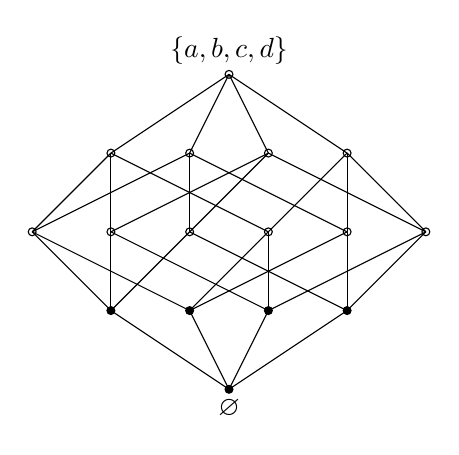
\begin{tikzpicture}
            \draw [fill] (0,0) circle [radius=0.05]; % \varnothin
            \node [below] at (0,0) {$\varnothing$};
            \draw (0,0) -- (-1.5,1);
            \draw (0,0) -- (-0.5,1);
            \draw (0,0) -- ( 0.5,1);
            \draw (0,0) -- ( 1.5,1);
            
            \draw[fill] (-1.5,1) circle [radius=0.05]; % {a}
            \draw[fill] (-0.5,1) circle [radius=0.05]; % {b}
            \draw[fill] (0.5,1) circle [radius=0.05]; % {c}
            \draw[fill] (1.5,1) circle [radius=0.05]; % {d}

            \draw (-2.5,2) -- (-1.5,1);
            \draw (-2.5,2) -- (-0.5,1);
            \draw (-1.5,2) -- (-1.5,1);
            \draw (-1.5,2) -- ( 0.5,1);
            \draw (-0.5,2) -- (-1.5,1);
            \draw (-0.5,2) -- ( 1.5,1);
            \draw ( 0.5,2) -- (-0.5,1);
            \draw ( 0.5,2) -- ( 0.5,1);
            \draw ( 1.5,2) -- (-0.5,1);
            \draw ( 1.5,2) -- ( 1.5,1);
            \draw ( 2.5,2) -- ( 0.5,1);
            \draw ( 2.5,2) -- ( 1.5,1);
            
            \draw[thin] (-2.5,2) circle [radius=0.05]; % {a,b}
            \draw[thin] (-1.5,2) circle [radius=0.05]; % {a,c}
            \draw[thin] (-0.5,2) circle [radius=0.05]; % {a,d}
            \draw[thin] (0.5,2) circle [radius=0.05]; % {b,c}
            \draw[thin] (1.5,2) circle [radius=0.05]; % {b,d}
            \draw[thin] (2.5,2) circle [radius=0.05]; % {c,d}

            \draw (-2.5,2) -- (-1.5,3);
            \draw (-2.5,2) -- (-0.5,3);
            \draw (-1.5,2) -- (-1.5,3);
            \draw (-1.5,2) -- ( 0.5,3);
            \draw (-0.5,2) -- (-0.5,3);
            \draw (-0.5,2) -- ( 0.5,3);
            \draw ( 0.5,2) -- (-1.5,3);
            \draw ( 0.5,2) -- ( 1.5,3);
            \draw ( 1.5,2) -- (-0.5,3);
            \draw ( 1.5,2) -- ( 1.5,3);
            \draw ( 2.5,2) -- ( 0.5,3);
            \draw ( 2.5,2) -- ( 1.5,3);
            
            \draw[thin] (-1.5,3) circle [radius=0.05]; % {a,b,c}
            \draw[thin] (-0.5,3) circle [radius=0.05]; % {a,b,d}
            \draw[thin] (0.5,3) circle [radius=0.05]; % {a,c,d}
            \draw[thin] (1.5,3) circle [radius=0.05]; % {b,c,d}

            \draw (-1.5,3) -- (0,4);
            \draw (-0.5,3) -- (0,4);
            \draw ( 0.5,3) -- (0,4);
            \draw ( 1.5,3) -- (0,4);
            
            \draw[thin] (0,4) circle [radius=0.05];
            \node [above] at (0,4) {$\{a,b,c,d\}$};
        \end{tikzpicture}
        \caption{Caption}
        \label{fig:ch01:sec06:prob5:1}
    \end{figure}
    
    \item 太麻烦了,不画了,懂意思就行.
\end{enumerate}
% problem 5 (end)

% section 等价关系. 商映射 (end)

\section{数学归纳法原理} % (begin)

\problem{1} % (begin)
\begin{quotation}
    令
    \[
    \begin{gathered}
        s(n) = \sin{\varphi} + \sin{2\varphi} + \cdots + \sin{n\varphi},\\
        c(n) = \cos{\varphi} + \cos{2\varphi} + \cdots + \cos{n\varphi}.
    \end{gathered}
    \]
    对 $n$ 作归纳证明公式
    \[
    s(n) = \frac{\sin{(n\varphi/2)}\sin((n+1)\varphi/2)}{\sin(\varphi/2)},
    c(n) = \frac{\sin{(n\varphi/2)}\cos((n+1)\varphi/2)}{\sin(\varphi/2)}.
    \]
\end{quotation}

\begin{proof}
    当 $n = 1$ 时
\end{proof}

% problem 1 (end)

% section 数学归纳法原理 (end)


\endinput


\end{document}
